\documentclass[journal]{IEEEtran} % use the `journal` option for ITherm conference style
\IEEEoverridecommandlockouts
% The preceding line is only needed to identify funding in the first footnote. If that is unneeded, please comment it out.
\usepackage{cite}
\usepackage{amsmath,amssymb,amsfonts}
\usepackage{algorithmic}
\usepackage{graphicx}
\usepackage{textcomp}
\usepackage{xcolor}
\graphicspath{ {./images/} }
\def\BibTeX{{\rm B\kern-.05em{\sc i\kern-.025em b}\kern-.08em
    T\kern-.1667em\lower.7ex\hbox{E}\kern-.125emX}}
\begin{document}

\title{LiDAR Object Tracking with Hardware Acceleration}


\author{%%%% author names
    \IEEEauthorblockN{McCain Boonma}\\% first author
    \IEEEauthorblockA{\textit{Northeastern University, Boston, USA}}\\% first affiliation
    \IEEEauthorblockA{boonma.m@northeastern.edu}
}

\maketitle

\begin{abstract}
This project presents an efficient solution for real-time processing and analysis of LiDAR data, leveraging FPGA-based hardware acceleration to perform clustering and a Kalman filter for object tracking. Utilizing a YDLiDAR X4 LiDAR sensor, distance data is collected and processed to identify clusters representing objects within the field of view. A PYNQ overlay is employed to accelerate clustering operations on a Xilinx FPGA platform, significantly improving the overall performance. The integration of a  Kalman filter enables tracking of detected clusters over time, allowing for the identification and monitoring of objects with constant velocities. Visualization of the processed data is achieved using polar plots with the Matplotlib library, providing a clear representation of the raw LiDAR data and the identified clusters.
\end{abstract}

\section{Introduction}
Light Detection and Ranging (LiDAR) sensors are widely used in various applications, including autonomous vehicles, robotics, and environmental monitoring. These sensors generate large amounts of data that require real-time processing to detect and track objects within their field of view. This paper presents an efficient solution for real-time processing and analysis of LiDAR data, leveraging FPGA-based hardware acceleration to perform clustering and a Kalman filter for object tracking. The proposed approach employs a number of hardware optimizations in the point clustering operation, resulting in significant improvements in overall performance. The processed data is visualized using polar plots , providing a clear representation of the raw LiDAR data and the identified clusters.

\section{System Overview}
This inclusive system (Fig \ref{fig:sysOverview}) includes LiDAR data collection, point clustering, and object tracking. The primary focus of this paper is the clustering algortihm implemented on the FPGA programmable logic via an overlay and the object tracking using a Kalman filter implemented on the FPGA processing system. 

\begin{figure}[h]
  \centering
  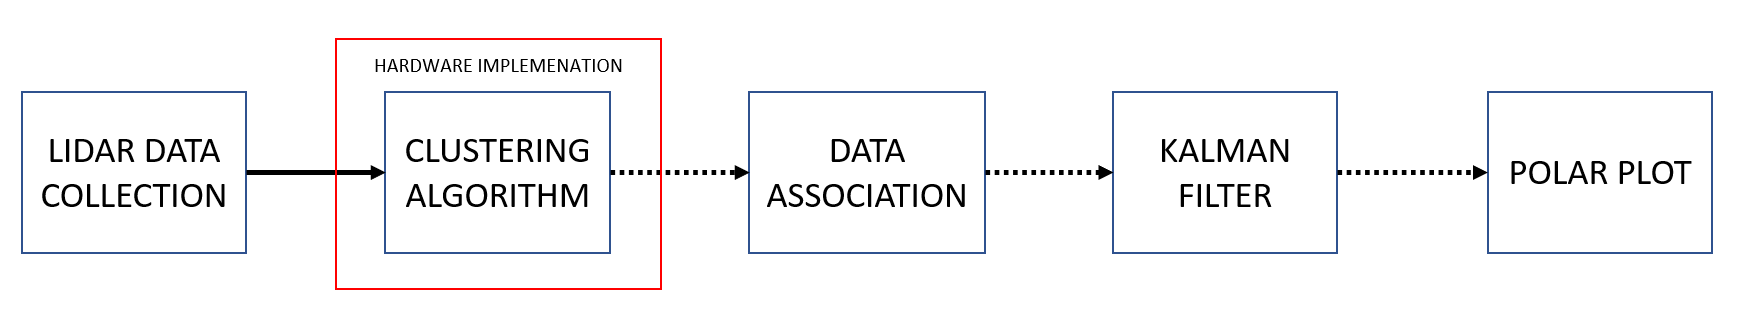
\includegraphics[width=0.5\textwidth]{sysOverview}
  \caption{System Overview}
  \label{fig:sysOverview}
\end{figure}

\subsection{LiDAR Data Collection}

The sensor's coordinate system is defined such that 0\textdegree originates from the center of the sensor assembly towards the LiDAR sensor's motor, with data collected in the clockwise direction (as shown in Fig. \ref{fig:polarLiDAR}). The sensor is connected to the processing system of the PYNQ Z2 via a USB port.

\begin{figure}[h]
  \centering
  \includegraphics[width=0.35\textwidth]{polarLiDAR}
  \caption{LiDAR Sensor Coordinate System Definition}
  \label{fig:polarLiDAR}
\end{figure}

 To control the LiDAR sensor and collect LiDAR data, the PyLidar3 library is utilized, which is a python 3 package. The LiDAR sensor is capable of a typical angle resolution of 0.50\textdegree at 7 Hz, but due to software limitations, the PyLidar3 library provides a resolution of only 1\textdegree regardless of the frequency. The collected data is returned in the form of a dictionary, comprising of 360 degrees of angle and corresponding distances in millimeters.\\


\subsection{Hardware Accelerated Point Clustering}

The point clustering operation was implemented on the programmable logic of the FPGA using an Overlay. To achieve this, the point clustering algorithm was developed in Vitis High-Level Synthesis (HLS). The LiDAR data is transferred from the FPGA processing system to the programmable logic through an AXI Stream interface, while the clustered data is transferred via a separate AXI Stream interface. The implemented clustering algorithm is based on the Density-Based Spatial Clustering of Applications with Noise (DBSCAN) algorithm, which is commonly utilized in LiDAR point clustering applications.\\

he clustering algorithm utilized in the proposed LiDAR object tracking system is based on the Density-Based Spatial Clustering of Applications with Noise (DBSCAN) algorithm. The DBSCAN algorithm takes three parameters: an array of distance data, the number of data points, and the maximum distance between two points in the same neighborhood (epsilon, $\epsilon$).

The DBSCAN algorithm starts by iterating over all the points in the input data array. For each unvisited point, the algorithm finds all its neighbors within a distance of $\epsilon$ and adds them to a cluster. The algorithm then expands the cluster by adding all reachable neighbors of each point in the cluster. The algorithm stops when no more points can be added to the cluster.

The distance calculation used in the DBSCAN algorithm takes into account the angle between the LiDAR points, which are represented as distances in an array. Given two points $p_1$ and $p_2$ in the array, the distance calculation between them is as follows:

\[
distance = \sqrt{(p_{1,x} - p_{2,x})^2 + (p_{1,y} - p_{2,y})^2}
\]

Where $p_{1,x}$ and $p_{2,x}$ are the distances of $p_1$ and $p_2$ from the LiDAR sensor along the horizontal axis, and $p_{1,y}$ and $p_{2,y}$ are the distances of $p_1$ and $p_2$ from the LiDAR sensor along the vertical axis. The distance calculation also involves converting the angles of the LiDAR points to radians, and using the sine and cosine functions to compute the horizontal and vertical distances respectively.

The implemented DBSCAN algorithm in the code snippet takes an array of distance data, the number of data points, and the maximum distance between two points in the same neighborhood (epsilon, $\epsilon$) as input. The algorithm iterates over all the points in the input array, finds all the neighbors of each unvisited point, and creates a new cluster if the point has enough neighbors. The algorithm then expands the cluster by adding all reachable neighbors, and continues until no more points can be added to the cluster.

After the raw LiDAR data set has been clustered, a Python helper function calculates each cluster's centroids and stores the clusters as centroid angle, centroid distance, and cluster size. 

%-----------------------------------------------------------------------------------------------------------------------------------------------------------------------------------------------------------------------------------------------
\subsection{Data Association - Scoring Algorithm}

In this particular application, the noise generated by the LiDAR sensor is significant and the size and location of the clusters varied significantly. Therefore, a robust data association algorithm was needed to match clusters from a previous frame in the current frame. To achieve this, a scoring algorithm was employed to match clusters between frames using the predictions from the Kalman filter.

In the first iteration, the master list was initialized by clustering the first dataset and storing it in the format of cluster centroid angle, cluster centroid distance, and cluster size. Each cluster was assigned a unique ID and stored in a master list. In subsequent iterations, a list of the current clusters, represented by their centroid and size, was generated. The data association algorithm iterated over each cluster in the master list and calculated a score against each cluster in the current frame's clusters. The current cluster with the lowest score was matched with the predicted state of the cluster under test from the Kalman filter.

The score was an aggregate score between the size of the cluster and the polar euclidean distance (PED), which is given by the following equation:

\[
\text{PED} = \sqrt{r_1^2 + r_2^2+2r_1r_2cos(\Delta\theta)}
\]

The aggregated score was calculated by multiplying the difference in cluster size and euclidean distance with double the weight assigned to the PED, as shown in the following equation:

\[ 
\text{Score} = \Delta \theta * 2  \text{PED}
\]

Due to the noise, it was possible for the master list to fluctuate in size. The data association algorithm took this into account. If there were more clusters in the current cluster list than in the master list, then the clusters not matched with a cluster from the master list were assigned a new unique ID. On the other hand, if there were more clusters in the master list than in the current cluster list, then the data association algorithm found and removed the excess clusters from the master list. The data association function matched each cluster in the master list, and in this case, multiple clusters in the master list could be matched to the same cluster from the current list. The data association function removed the matched clusters with the highest score, i.e., the worst fit.

The data association function replaced the master list with the newly updated lists. Each matched cluster retains the unique ID of the cluster the scoring algorithm determined was the best fit based on the cluster size and euclidean distance between the centroids. The Kalman filter is then updated with the matched cluster's measurements, improving the accuracy of its predictions in subsequent iterations.

%-----------------------------------------------------------------------------------------------------------------------------------------------------------------------------------------------------------------------------------------------

\subsection{Kalman Filter for Cluster Tracking}

In this section, we will focus on the application of the Kalman filter for tracking clusters in addition to the data association. As the clusters in the master list may vary signficantly from frame to frame, implementing the Kalman filter reduces the noise and gives a consistent and reliable view into the true location and size of a cluster. The Kalman filter is a recursive algorithm that provides an optimal estimate of the state of a dynamic system given noisy measurements. In the context of LiDAR cluster tracking, the dynamic system represents the clusters' positions and sizes, while the noisy measurements correspond to noisy LiDAR data collection.

\subsubsection{Kalman Filter Overview}

The Kalman filter consists of two main steps: prediction and update. Given the previous state estimate $x_{k-1|k-1}$ and its associated uncertainty covariance $P_{k-1|k-1}$, the filter first predicts the state at the next time step $k$ using a state transition model:

\[
x_{k|k-1} = F_k x_{k-1|k-1}
\]

where $F_k$ is the state transition matrix. The uncertainty covariance of the predicted state is also updated:

\[
P_{k|k-1} = F_k P_{k-1|k-1} F_k^T + Q_k
\]

where $Q_k$ is the process noise covariance.

Next, the filter incorporates a new measurement $z_k$ to update the predicted state. First, the measurement is compared to the predicted state using the measurement model:

\[
y_k = z_k - H_k x_{k|k-1}
\]

where $H_k$ is the measurement matrix. Then, the Kalman gain is computed:

\[
K_k = P_{k|k-1} H_k^T (H_k P_{k|k-1} H_k^T + R_k)^{-1}
\]

where $R_k$ is the measurement noise covariance. The Kalman gain is used to update the state estimate:

\[
x_{k|k} = x_{k|k-1} + K_k y_k
\]

Finally, the uncertainty covariance of the updated state is computed:

\[
P_{k|k} = (I_6 - K_k H_k) P_{k|k-1}
\]

These steps are repeated for each new measurement to provide continuous tracking and prediction of the clusters in the LiDAR point cloud.

\subsubsection{Applying the Kalman Filter to Cluster Tracking}

To apply the Kalman filter to cluster tracking, we perform the following steps for each time step:\\

1. For each unique cluster in the master list, predict its state at the current time step using its associated Kalman filter:

   \[
   \mathrm{kf.predict()} \Rightarrow x_{k|k-1}
   \]

2. Match the predicted cluster states with the detected clusters in the current frame. In this case, we use the previously mentioned data association function to find the optimal assignment between predicted and detected clusters based on their Euclidean distance and cluster size.\\

3. For each matched pair of predicted and detected clusters, update the associated Kalman filter with the new measurement:

   \[
   \mathrm{kf.update}(z_k) \Rightarrow x_{k|k}, P_{k|k}
   \]

4. For each unmatched detected cluster, create a new entry in the master list, and initialize a new Kalman filter with the initial state set to the detected cluster's properties:

\[
x_0 = \begin{bmatrix}
\text{centroid\_angle} \\
\text{centroid\_distance} \\
\text{cluster\_size} \\
0 \\
0 \\
0\\
\end{bmatrix}
\]

5. For each unmatched predicted cluster, consider removing it from the master list based on a predefined criterion, such as a maximum allowed time without detection or a maximum allowed uncertainty in the state estimate.

\subsubsection{Parameter Selection}

For the Kalman filter to provide accurate and reliable tracking, it is crucial to select appropriate values for the state transition, measurement, and noise covariance matrices. In our implementation, the state transition matrix $F_k$ is defined as:

\[
F_k = \begin{bmatrix}
1 & 0 & 0 & 1 & 0 & 0 \\
0 & 1 & 0 & 0 & 1 & 0 \\
0 & 0 & 1 & 0 & 0 & 1 \\
0 & 0 & 0 & 1 & 0 & 0 \\
0 & 0 & 0 & 0 & 1 & 0 \\
0 & 0 & 0 & 0 & 0 & 1
\end{bmatrix}
\]

This matrix assumes that the clusters move with constant velocity in the angle-distance space. The measurement matrix $H_k$ is defined as:

\[
H_k = \begin{bmatrix}
1 & 0 & 0 & 0 & 0 & 0 \\
0 & 1 & 0 & 0 & 0 & 0 \\
0 & 0 & 1 & 0 & 0 & 0
\end{bmatrix}
\]

which extracts the angle, distance, and size components from the state vector.

The process noise covariance $Q_k$ is defined using the discrete-time white noise model:

\[
Q_k = Q_{\text{continuous}}(3, dt, \sigma^2) =
\begin{bmatrix}
\frac{1}{3}dt^3 & \frac{1}{2}dt^2 \\
\frac{1}{2}dt^2 & dt
\end{bmatrix} \sigma^2
\]

where $dt$ is the time step and $\sigma^2$ is the variance of the continuous-time white noise process. In our implementation, we set $dt = 1$ and $\sigma^2 = 0.1$.

\subsection{Performance Considerations}

When applying the Kalman filter to LiDAR cluster tracking, several factors can impact its performance, including:

\textbf{Measurement noise}: The accuracy of the LiDAR point cloud data can affect the Kalman filter's ability to track clusters. Higher measurement noise levels may result in increased uncertainty in the state estimate and less reliable tracking.

\textbf{Cluster dynamics}: The dynamics of the clusters in the LiDAR point cloud, such as their motion and size changes, can also impact the performance of the Kalman filter. If the cluster dynamics are not accurately represented by the state transition matrix and the process noise covariance, the filter's performance may be degraded.

\textbf{Initialization}: The initial state of the Kalman filter can have a significant impact on its performance. If the initial state is far from the true state of the cluster, it may take the filter several time steps to converge to the correct state. To improve performance, it is crucial to initialize the filter with a reasonable estimate of the cluster's initial properties.

\textbf{Parameter tuning}: The parameters of the Kalman filter, such as the process noise covariance and the measurement noise covariance, need to be tuned based on the specific application and the characteristics of the LiDAR point cloud data. Poorly chosen parameters can lead to suboptimal tracking performance or increased uncertainty in the state estimates.

\textbf{Computational complexity}: The computational complexity of the Kalman filter can be an issue when tracking a large number of clusters in real-time. Optimizations, such as parallel processing or the use of more efficient algorithms for updating the state estimates, can help mitigate this issue.

%-----------------------------------------------------------------------------------------------------------------------------------------------------------------------------------------------------------------------------------------------


\subsection{Visualization}

Visualization plays a crucial role in analyzing the performance of the LiDAR data processing pipeline and understanding the identified clusters and their tracked positions. This project uses the Matplotlib library to generate polar plots for the visualization of raw LiDAR data, identified clusters, and tracked clusters.

Two polar plots are created for each iteration of the processing loop:
\begin{itemize}

\item Raw Data Plot: This plot displays the distance values collected by the LiDAR sensor at different angles. It helps to visualize the raw LiDAR data and understand the environment.

\item Clustered Data Plot: This plot shows the identified clusters and the predicted locations as described by the Kalman filter, represented by red crosses. It is useful for evaluating the performance of the clustering algorithm, data association algorithm, and Kalman Filtering.

\end{itemize}

The update\_plot function is responsible for updating the polar plots with the raw and clustered data. It first clears the axes, then plots the data points on the respective polar plots, and finally updates the plot titles and limits. The function also calls the data\_association function to perform data association and updates the Kalman Filter between the current and previous clusters.

\section{Implementation}

\subsection{Hardware}
The clustering operation is an ideal candidate for hardware acceleration due to its computationally intensive nature and the ability to parallelize the algorithm. By grouping distances into clusters using a straightforward algorithm, hardware acceleration can significantly improve performance. The functionality of the clustering operation was verified by comparing the clusters generated by the hardware implementation to those generated by a software implementation using the same data.

\subsection{Software}
The Kalman Filter and data association are potential candidates for hardware acceleration. However, due to the intricacy of their mathematical algorithms and time constraints, hardware testing would have been excessively time-consuming. Thus, software implementation was chosen to expedite the development process.

\subsection{Implementation Overview}

The entire processing pipeline is implemented in a Jupyter Notebook, using the PYNQ library for FPGA acceleration, PyLidar3 library for LiDAR data collection, and the Matplotlib library for data visualization. The constant velocity Kalman filter is implemented using the pykalman library.

First, the LiDAR sensor is initialized and connected to the Linux-based system. Then, the PYNQ overlay is loaded onto the FPGA, and the input and output buffers are allocated for the clustering operation. The processing loop iterates for a user-defined number of times, performing the following steps in each iteration:

\begin{enumerate}
\item Collect distance data from the LiDAR sensor.
\item Perform the FPGA-based clustering operation on the collected data.
\item Update the constant velocity Kalman filter for the detected clusters.
\item Perform data association between the current and previous clusters.
\item Update the polar plots with the raw and clustered data.
\end{enumerate}

Upon completion of the processing loop, the LiDAR sensor is disconnected, and the program exits.


\section{Results and Discussion}

The proposed solution demonstrates the effectiveness of FPGA-based hardware acceleration for real-time processing and analysis of LiDAR data. By offloading the computationally intensive clustering operation onto the FPGA, the overall performance of the system is improved.

The polar plot visualization provides a clear representation of the raw LiDAR data and the identified clusters, facilitating the analysis of the system's performance. The data association algorithm successfully matches the detected clusters with the tracked objects, ensuring that the state of the constant velocity Kalman filter is updated correctly.

The data association portion of the project is currently facing major issues, rendering it non-operational (work is still ongoing to address these issues). Consequently, the Kalman filter is only able to return the current mean position of a cluster, and it is not yet behaving as a fully functional Kalman Filter. Despite these issues, communication between the LiDAR sensor and the PYNQ board is reliable, and connectivity issues are rare. While the clustering operation has not been benchmarked against the initial software implementation, it is operating reliably. However, plotting the data remains the slowest part of the pipeline.

Despite these challenges, the project is capable of connecting to a LiDAR sensor and successfully clustering LiDAR data. Additionally, groundwork has been laid for a functioning Kalman Filter, which will enable accurate tracking of objects with constant velocities.

\section{Conclusion}

This paper presents an efficient solution for real-time processing and analysis of LiDAR data using FPGA-based hardware acceleration. The proposed approach employs a YDLiDAR X4 LiDAR sensor for data collection and a Xilinx FPGA platform for acceleration, achieving significant improvements in overall performance. The integration of a constant velocity Kalman filter enables accurate tracking of detected clusters over time, while the data visualization using polar plots provides a clear representation of the raw LiDAR data and the identified clusters. Future work may explore the use of more advanced clustering algorithms and tracking filters to further enhance the performance of the system, as well as the implementation of additional features such as object classification and prediction.

\begin{thebibliography}{00}
    \bibitem{b1} L, Mallidi, "PyLidar3," GitHub, 2020, url: https://github.com/lakshmanmallidi/PyLidar3
    \bibitem{b2} K, Konstantinidis, "Detection and Tracking of Moving Objects with 2D LiDAR," GitHub, 2022, url: https://github.com/kostaskonkk/datmo
    \bibitem{b3} K. Beomseong, C. Baehoon, Y. Minkyun, K. Hyunju, K. Euntai. (2014). Robust Object Segmentation Using a Multi-Layer Laser Scanner. Sensors (Basel, Switzerland). 14. 20400-18. 10.3390/s141120400. 
    \bibitem{b4} R. Su, J. Tang, J. Yuan and Y. Bi, "Nearest Neighbor Data Association Algorithm Based on Robust Kalman Filtering," 2021 2nd International Symposium on Computer Engineering and Intelligent Communications (ISCEIC), Nanjing, China, 2021, pp. 177-181, doi: 10.1109/ISCEIC53685.2021.00044.
    \bibitem{b5} N. Baisa, "Derivation of a Constant Velocity Motion Model for Visual Tracking," arXiv, 2020, doi: 10.48550/ARXIV.2005.00844

\end{thebibliography}

\end{document}
